\documentclass[10pt,a4paper]{report}
\usepackage[utf8]{inputenc}
\usepackage[T1]{fontenc}
\usepackage[english]{babel}
\usepackage{geometry}
\usepackage{graphicx}
\usepackage{hyperref}
\usepackage{listings}
\usepackage{xcolor}
\usepackage{longtable}
\usepackage{booktabs}
\usepackage{fancyhdr}
\usepackage{titlesec}
\usepackage{enumitem}
\usepackage{url}
\usepackage{tabularx}
\usepackage{multirow}
\usepackage{tikz}
\usetikzlibrary{shapes.geometric, arrows.meta, positioning, fit, backgrounds}

% Page geometry
\geometry{
    left=2.5cm,
    right=2.5cm,
    top=3cm,
    bottom=3cm,
    headheight=15pt
}

% Hyperref setup
\hypersetup{
    colorlinks=true,
    linkcolor=blue,
    filecolor=magenta,
    urlcolor=cyan,
    citecolor=green,
    pdftitle={Final Project Report - The Hive Platform},
    pdfauthor={Sena Oz, Aysenur Unal, Kenan Altunbas, Yusuf Savas}
}

% Code listing setup
\lstset{
    basicstyle=\ttfamily\small,
    breaklines=true,
    frame=single,
    numbers=left,
    numberstyle=\tiny\color{gray},
    backgroundcolor=\color{gray!10},
    keywordstyle=\color{blue},
    commentstyle=\color{green!60!black},
    stringstyle=\color{red},
    showspaces=false,
    showstringspaces=false
}

% Header and footer
\pagestyle{fancy}
\fancyhf{}
\fancyhead[L]{\leftmark}
\fancyhead[R]{\thepage}
\fancyfoot[C]{The Hive Platform --- Final Project Report}

% Title formatting
\titleformat{\chapter}[display]
{\normalfont\Large\bfseries}{\chaptertitlename\ \thechapter}{20pt}{\Large}
\titlespacing*{\chapter}{0pt}{50pt}{40pt}

% Title page information
\title{
    \vspace*{2cm}
    \Huge\textbf{Final Project Report}\\
    \vspace{1cm}
    \Large\textbf{The Hive Platform}\\
    \large Community Service Exchange TimeBank Platform
    \vspace{2cm}
}

\author{
    \Large\textbf{Sena Oz \quad Ay\c{s}enur \"{U}nal}\\
    \Large\textbf{Kenan Altunba\c{s} \quad Yusuf Sava\c{s}}\\
    \vspace{0.5cm}
    \large Software Engineering MS Program\\
    Bo\u{g}azi\c{c}i University\\
    \vspace{1cm}
    \large\textbf{SWE 574}\\
    Software Development Practice\\
    Spring 2026
}

\date{
    \vspace{1cm}
    May 2026\\
    \vspace{2cm}
    \begin{tabular}{ll}
        \textbf{Git Repository:}  & \url{https://github.com/senaoz/SWE-574}\\
        \textbf{Git Tag:}         & \texttt{customer-milestone-2}\\
        \textbf{Deployment URL:}  & \url{https://swe.gnahh5.easypanel.host}\\
        \textbf{Backend API:}     & \url{https://backend-swe.gnahh5.easypanel.host/docs}\\
    \end{tabular}
}

\begin{document}

% Title page
\maketitle
\thispagestyle{empty}

% Honor Code Page
\newpage
\thispagestyle{empty}
\vspace*{2cm}

\begin{center}
    \large\textbf{HONOR CODE}
\end{center}

\vspace{1cm}

\large
Related to the submission of all the project deliverables for the SWE 574 Spring 2026 semester project reported in this report, we \textbf{Sena Oz, Ay\c{s}enur \"{U}nal, Kenan Altunba\c{s}, and Yusuf Sava\c{s}} declare that:

\begin{itemize}[leftmargin=0.5cm]
    \item We are students in the Software Engineering MS program at Bo\u{g}azi\c{c}i University and are registered for SWE 574 course during the Spring 2026 semester.

    \item All the material that we are submitting related to our project (including but not limited to the project repository, the final project report, and supplementary documents) have been exclusively prepared by the team members named above.

    \item We have prepared this material as a team without the assistance of anyone else with the exception of permitted peer assistance, which we have explicitly disclosed in this report.

    \item We have used AI tools (Claude, ChatGPT, Gemini) as development assistants, which we have fully disclosed in the AI Use Declaration document.

    \item All third-party software and libraries used have been properly attributed and their licenses respected, as documented in the Third-Party Software document.
\end{itemize}

\vspace{1cm}

\begin{center}
\begin{tabular}{p{6cm} p{6cm}}
    \textbf{Sena Oz} & \textbf{Ay\c{s}enur \"{U}nal} \\[1.5cm]
    \rule{5.5cm}{0.4pt} & \rule{5.5cm}{0.4pt} \\
    Signature & Signature \\[1.5cm]
    \textbf{Kenan Altunba\c{s}} & \textbf{Yusuf Sava\c{s}} \\[1.5cm]
    \rule{5.5cm}{0.4pt} & \rule{5.5cm}{0.4pt} \\
    Signature & Signature \\
\end{tabular}
\end{center}

\newpage
\tableofcontents
\newpage
\listoffigures
\newpage
\listoftables

% =========================================================
\chapter{List of Deliverables}
% =========================================================

This chapter lists all project deliverables submitted across the two milestones and the final report.

\section{Milestone 1 Deliverables}

Milestone 1 was delivered on 9 March 2026. All deliverables are available on the project GitHub Wiki.

\begin{table}[h]
    \centering
    \begin{tabularx}{\textwidth}{|l|X|}
        \hline
        \textbf{Deliverable}                  & \textbf{Location}                                                                          \\
        \hline
        Software Requirements Specification   & \url{https://github.com/senaoz/SWE-574/wiki/SRS}                                           \\
        \hline
        UML Diagrams                          & \url{https://github.com/senaoz/SWE-574/wiki/UML-Diagrams}                                  \\
        \hline
        Scenarios \& Mockups                  & \url{https://github.com/senaoz/SWE-574/wiki/Scenarios-\&-Mockups}                          \\
        \hline
        Project Plan                          & \url{https://github.com/senaoz/SWE-574/wiki}                                               \\
        \hline
        Communication Plan                    & \url{https://github.com/senaoz/SWE-574/wiki/Communication-Plan}                            \\
        \hline
        Responsibility Assignment Matrix      & \url{https://github.com/senaoz/SWE-574/wiki/Responsibility-Assignment-Matrix-(RACI)}        \\
        \hline
        Weekly Reports \& Meeting Notes       & \url{https://github.com/senaoz/SWE-574/wiki/Meeting-Notes}                                 \\
        \hline
        Milestone 1 Report                    & \url{https://github.com/senaoz/SWE-574/blob/main/reports/m1\_group3.md}                    \\
        \hline
        GitHub Release                        & \url{https://github.com/senaoz/SWE-574/releases/tag/customer-milestone-1}                  \\
        \hline
    \end{tabularx}
    \caption{Milestone 1 Deliverables}
\end{table}

\section{Milestone 2 Deliverables}

Milestone 2 was delivered on 13 April 2026. All deliverables are available on the project GitHub Wiki and repository.

\begin{table}[h]
    \centering
    \begin{tabularx}{\textwidth}{|l|X|}
        \hline
        \textbf{Deliverable}                  & \textbf{Location}                                                                          \\
        \hline
        Updated SRS                           & \url{https://github.com/senaoz/SWE-574/wiki/SRS}                                           \\
        \hline
        Architecture \& Design Docs           & \url{https://github.com/senaoz/SWE-574/wiki/UML-Diagrams}                                  \\
        \hline
        Deployment (live)                     & \url{https://swe.gnahh5.easypanel.host}                                                    \\
        \hline
        Backend API Documentation             & \url{https://backend-swe.gnahh5.easypanel.host/docs}                                       \\
        \hline
        Milestone 2 Report                    & \url{https://github.com/senaoz/SWE-574/blob/main/reports/m2\_group3.md}                    \\
        \hline
        GitHub Release                        & \url{https://github.com/senaoz/SWE-574/releases/tag/customer-milestone-2}                  \\
        \hline
    \end{tabularx}
    \caption{Milestone 2 Deliverables}
\end{table}

\section{Final Deliverables}

\begin{table}[h]
    \centering
    \begin{tabularx}{\textwidth}{|l|X|}
        \hline
        \textbf{Deliverable}                  & \textbf{Location / Description}                                                            \\
        \hline
        Final Project Report (this document)  & \texttt{reports/latex/main.pdf} in repository                                              \\
        \hline
        Source Code Repository                & \url{https://github.com/senaoz/SWE-574}                                                    \\
        \hline
        Live Web Deployment                   & \url{https://swe.gnahh5.easypanel.host}                                                    \\
        \hline
        Android APK                           & \texttt{apk/} directory in repository root                                                 \\
        \hline
        Demo Video                            & \textit{[TBD --- link to be added before submission. Maximum 5 minutes.]}                  \\
        \hline
    \end{tabularx}
    \caption{Final Deliverables}
\end{table}

% =========================================================
\chapter{Test Credentials and Demo}
% =========================================================

\section{Demo Video}

\textit{[TBD --- A demo video of no more than 5 minutes will be provided before final submission. It will walk through the core user workflow: registration, service creation, service discovery, join request, approval, chat, transaction completion, and TimeBank credit update.]}

\section{Test User Accounts}

The following test accounts are available on the live deployment for evaluation:

\begin{table}[h]
    \centering
    \begin{tabular}{|l|l|l|}
        \hline
        \textbf{Role}       & \textbf{Email}                    & \textbf{Password}    \\
        \hline
        Admin               & \texttt{tazeyta@gmail.com}        & \texttt{Password123} \\
        \hline
        Regular User        & \texttt{elif.sahin@example.com}   & \texttt{Password123} \\
        \hline
        Regular User        & \texttt{mehmet.demir@example.com} & \texttt{Password123} \\
        \hline
    \end{tabular}
    \caption{Test User Credentials}
\end{table}

\section{Deployment Information}

\begin{itemize}
    \item \textbf{Live Application:} \url{https://swe.gnahh5.easypanel.host}
    \item \textbf{Backend API:} \url{https://backend-swe.gnahh5.easypanel.host}
    \item \textbf{API Documentation (Swagger):} \url{https://backend-swe.gnahh5.easypanel.host/docs}
    \item \textbf{Git Repository:} \url{https://github.com/senaoz/SWE-574}
    \item \textbf{Git Tag:} \texttt{customer-milestone-2}
\end{itemize}

\section{Testing Instructions}

\begin{enumerate}
    \item Navigate to \url{https://swe.gnahh5.easypanel.host}
    \item Log in with a test account from the table above
    \item Key features to test:
          \begin{itemize}
              \item Service creation (offers and needs)
              \item Service discovery, search, and map view
              \item Join request workflow (apply, approve, reject)
              \item Transaction completion with dual confirmation
              \item Chat functionality
              \item TimeBank balance and history
              \item Forum (discussions, events, communities)
              \item Badges and ratings
              \item Admin panel (using admin account)
          \end{itemize}
\end{enumerate}

% =========================================================
\chapter{Project Overview}
% =========================================================

\section{Introduction}

The Hive Platform is a community-oriented service exchange platform based on the TimeBank concept, where one hour of service equals one hour of credit. The platform enables community members to offer services they can provide, request services they need, and exchange services using a TimeBank credit system.

The project was developed as part of the SWE 574 Software Development Practice course at Bo\u{g}azi\c{c}i University, Spring 2026 semester.

\section{Key Features}

\begin{itemize}
    \item \textbf{Service Exchange:} Users create service offers and needs; join requests, approvals, and dual-confirmation transactions manage the exchange workflow.
    \item \textbf{TimeBank System:} Credits in hours track contributions and consumption. Starting balance: 3 hours; maximum: 10 hours.
    \item \textbf{Interactive Map:} Google Maps API visualizes service locations with privacy-preserving fuzzed coordinates.
    \item \textbf{Forum:} Discussions, events, and community spaces for community interaction.
    \item \textbf{Communities:} User-created groups with posts, events, and member management.
    \item \textbf{Chat:} Messaging between service participants (auto-created on approval).
    \item \textbf{Badges:} Automatically awarded based on objective milestones.
    \item \textbf{Ratings:} Post-exchange star ratings with feedback labels and image attachments.
    \item \textbf{Recommendations:} Tag-based personalized service recommendations.
    \item \textbf{Admin Panel:} Moderation, user management, analytics, and report handling.
    \item \textbf{Android App:} Native Android client (Kotlin/Jetpack Compose) sharing the same backend.
\end{itemize}

\section{Technology Stack}

\subsection{Frontend (Web)}

React 18 with TypeScript, built with Vite. UI components from Radix UI, styled with Tailwind CSS. Google Maps API for map interaction. React Query for server state; Axios for API calls.

\subsection{Backend}

FastAPI (Python 3.11) with async Motor driver for MongoDB. JWT authentication (HS256, 30-minute expiry). Pydantic models for request/response validation. Content moderation via \texttt{alt-profanity-check}. WikiData API for semantic tag suggestions.

\subsection{Database}

MongoDB 7 with geospatial (2dsphere) indexes on service locations. Motor async driver. 15 collections including users, services, transactions, forum, communities, and notifications.

\subsection{Android App}

Kotlin with Jetpack Compose, MVVM architecture, Hilt DI, Retrofit + Moshi, DataStore for token persistence.

\subsection{Infrastructure}

Docker + Docker Compose for full-stack containerization. Nginx serves the React SPA in production. Deployed on EasyPanel via GitHub Actions CI/CD.

\section{Architecture}

The system follows a three-tier architecture:
\begin{itemize}
    \item \textbf{Client tier:} React SPA (web) and Android app
    \item \textbf{API tier:} FastAPI REST API with JWT authentication, served behind Nginx
    \item \textbf{Data tier:} MongoDB 7 database
\end{itemize}

See Chapter~\ref{chap:design} for detailed architecture diagrams.

% =========================================================
\chapter{Software Requirements Specification}
% =========================================================

\section{Introduction}

\subsection{Purpose}

This SRS defines the functional and non-functional requirements for The Hive platform, a community-oriented web application for the mutual exchange of services based on time. Based on IEEE 830.

\subsection{Product Scope}

The Hive is a virtual public space where individuals exchange services non-commercially. Its objectives:
\begin{itemize}
    \item Provide a map-based interface for posting and discovering service Offers and Needs
    \item Enable semantic tagging for discovery and organization
    \item Maintain a TimeBank system where time, not money, serves as the unit of value
    \item Support profile-based community trust, comments, and contribution histories
    \item Allow users to connect, communicate, and schedule services
\end{itemize}

\textit{Note: The SRS was authored during the design phase. The final implementation uses FastAPI + MongoDB rather than Django/Spring Boot + PostgreSQL as originally planned. All functional requirements were implemented as specified.}

\subsection{User Classes}

\begin{table}[h]
    \centering
    \begin{tabularx}{\textwidth}{|l|X|X|}
        \hline
        \textbf{User Class}   & \textbf{Description}                                                                  & \textbf{Privileges}                                              \\
        \hline
        Regular User          & General community member who posts, offers, and participates in exchanges.            & Create offers/needs, message, comment, report content.           \\
        \hline
        Moderator             & Trusted user responsible for community quality and handling reports.                  & Remove content, review flagged posts, manage comments.           \\
        \hline
        Admin                 & Platform operator with full control over system health, data, and governance.         & Full control: manage users, moderators, tags, reports.           \\
        \hline
    \end{tabularx}
    \caption{User Classes}
\end{table}

\section{Functional Requirements}

\subsection{FR--1: User Registration and Authentication}
\begin{itemize}
    \item FR--1.1 The system shall allow users to register with a unique username, email, and password.
    \item FR--1.2 The system shall validate email format and password complexity upon registration.
    \item FR--1.3 The system shall provide login and logout functionality.
    \item FR--1.4 The system shall encrypt all stored passwords using secure hashing.
    \item FR--1.5 The system shall provide session-based authentication for authorized access.
    \item FR--1.6 The system shall prompt users to select at least one interest (semantic tag) during registration.
\end{itemize}

\subsection{FR--2: Profile Management}
\begin{itemize}
    \item FR--2.1 Each user shall have a public profile displaying interest tags, total hours given/received, badges, completed exchanges, and comments.
    \item FR--2.2 The system shall display a user's current TimeBank balance on their profile.
    \item FR--2.3 The profile shall show completed exchanges.
    \item FR--2.4 Users shall be able to edit personal details such as display name and description.
    \item FR--2.5 The system shall automatically moderate user descriptions using keyword filters.
    \item FR--2.6 The system shall display the user's selected interests on their public profile using a tag format.
    \item FR--2.7 Users shall be able to add or remove interests from their profile at any time.
    \item FR--2.8 \textit{(Mobile)} The system shall allow users to upload or update their profile picture using the device camera or gallery.
    \item FR--2.9 \textit{(Mobile)} Profile editing interfaces shall use bottom sheets.
\end{itemize}

\subsection{FR--3: Offer and Need Management}
\begin{itemize}
    \item FR--3.1 The system shall allow users to create Offers and Needs containing: title, description, tags, approximate location, city (auto-detected), duration, remote/in-person indicator, and capacity (default 1).
    \item FR--3.2 Users shall be able to edit offers.
    \item FR--3.3 Offers and needs shall be shown on the profile after completion.
    \item FR--3.4 Users shall be able to mark their offers as remote.
    \item FR--3.5 Users shall assign one or more semantic tags when posting.
    \item FR--3.6 The system shall track accepted participants and shall not allow exceeding declared capacity.
    \item FR--3.7 Capacity may be increased while active; it shall not be decreased below the current accepted count.
    \item FR--3.8 \textit{(Mobile)} Users shall be able to attach up to 3 photos to any Offer or Need post.
\end{itemize}

\subsection{FR--4: Availability}
\begin{itemize}
    \item FR--4.2 A requester viewing an offer shall be able to select available hours for scheduling.
\end{itemize}

\subsection{FR--5: Handshake Mechanism}
\begin{itemize}
    \item FR--5.1 When a user applies to a need, the system shall prompt for an optional short message.
    \item FR--5.2 The application shall be marked as pending until the provider explicitly approves or rejects.
    \item FR--5.3 Once accepted, the exchange shall be confirmed and become active.
    \item FR--5.4 The system shall record the date and duration of the confirmed exchange in both users' histories.
    \item FR--5.5 A Need or Offer may accept multiple participants up to its capacity.
    \item FR--5.6 When accepted participants reach capacity, the post shall be marked Full.
    \item FR--5.7 \textit{(Mobile)} The system shall send push notifications via FCM for new handshake requests.
\end{itemize}

\subsection{FR--6: Messaging System}
\begin{itemize}
    \item FR--6.1 The system shall allow text-based communication between participants in an active exchange.
    \item FR--6.2 Messages shall be private and visible only to participants.
    \item FR--6.3 Messaging shall be disabled after an exchange is marked complete.
    \item FR--6.4 \textit{(Mobile)} The app shall support push notifications for incoming private messages.
    \item FR--6.5 When a service transitions to Active, the system shall automatically create a group chat room with all confirmed participants and the provider.
    \item FR--6.6 Each message in a group chat room shall display the sender's profile picture.
\end{itemize}

\subsection{FR--7: TimeBank System}
\begin{itemize}
    \item FR--7.1 Each user shall start with an initial balance of 3 hours.
    \item FR--7.2 The system shall update TimeBank balance automatically on exchange completion: provider gains hours, requester loses hours.
    \item FR--7.3 Users shall not exceed a balance of +10 hours without opening a Need.
    \item FR--7.4 The system shall calculate an effective maximum balance using worst-case pending transactions.
    \item FR--7.5 All TimeBank transactions shall be logged for auditability.
    \item FR--7.6 For exchanges with multiple participants, the system shall record a separate transaction per participant.
    \item FR--7.7 Anti-hoarding rule: a provider facilitating multiple requesters earns at most the actual session duration once.
    \item FR--7.8 The system shall only allow whole-hour transactions; fractional hours are not supported.
\end{itemize}

\subsection{FR--8: Tagging and Search}
\begin{itemize}
    \item FR--8.1 The system shall integrate with the Wikidata API to suggest and validate semantic tags.
    \item FR--8.2 Users shall be able to search and filter content by existing tags.
    \item FR--8.3 Search filters shall only display tags currently active in the database.
    \item FR--8.4 \textit{(Mobile)} Filtering interfaces shall use bottom sheets.
\end{itemize}

\subsection{FR--9: Map-Based Visualization}
\begin{itemize}
    \item FR--9.1 The system shall display Offers and Needs on an interactive map.
    \item FR--9.2 The system shall visualize locations using a randomized offset (fuzzing) to prevent exact address exposure.
    \item FR--9.3 The map shall visually differentiate between Offers and Needs.
    \item FR--9.4 The map shall allow filtering by distance, tag, and service type.
    \item FR--9.5 \textit{(Mobile)} The app shall include a ``Near to Me'' feature using device GPS.
\end{itemize}

\subsection{FR--10: Comment and Feedback System}
\begin{itemize}
    \item FR--10.1 After completing an exchange, both participants may leave a comment on each other's profile.
    \item FR--10.2 All comments shall pass through automated text moderation filters.
    \item FR--10.3 Comments shall be publicly visible on profiles.
    \item FR--10.4 The system shall allow users to provide a numerical rating (1--5 stars) alongside their comment.
    \item FR--10.5 The average rating score shall be displayed on the user's public profile.
    \item FR--10.6 The system shall provide predefined feedback labels (e.g., Helpful, Kind, Punctual, Communicative, Skilled); up to 5 labels per submission.
    \item FR--10.7 Selected feedback labels shall be displayed alongside the comment and rating.
    \item FR--10.8 Users shall be able to attach up to 3 images to a feedback submission.
    \item FR--10.9 Attached feedback images shall be displayed in a gallery format on the recipient's profile.
\end{itemize}

\subsection{FR--11: Reporting and Moderation}
\begin{itemize}
    \item FR--11.1 Users shall be able to report inappropriate content or behavior.
    \item FR--11.2 Moderators shall review and take action on reports.
    \item FR--11.3 Admins shall have the ability to manage moderators and system-wide settings.
    \item FR--11.4 Reports and their resolutions shall be logged in the system.
\end{itemize}

\subsection{FR--12: Completion and Transparency}
\begin{itemize}
    \item FR--12.1 Completed content shall be visible under each user's public profile.
    \item FR--12.2 Users shall be able to view their past exchanges, including dates and durations.
\end{itemize}

\subsection{FR--13: Badges}
\begin{itemize}
    \item FR--13.1 The system shall award badges automatically based on objective criteria.
    \item FR--13.2 Earned badges shall be displayed on the user's profile and next to display names on cards.
    \item FR--13.3 Badge eligibility shall be recalculated dynamically. Milestone badges remain once earned.
    \item FR--13.4 The initial badge set includes (minimum): Newcomer, Polished Wings, Pollen Collector, Nectar Expert, Sweet Taste, Honeycomb Star, Queen's Choice, Honey Maker, Worker Bee, Pollinator Bee, Elite Forager, Queen Bee.
    \item FR--13.5 The system shall provide an admin-visible catalog of badge definitions.
    \item FR--13.6 Badges shall not affect search ranking or access rights.
\end{itemize}

\subsection{FR--14: Active Items Management}
\begin{itemize}
    \item FR--14.1 The system shall provide a dedicated page for authenticated users to manage ongoing participation.
    \item FR--14.2 All active and inactive services shall present on the profile.
    \item FR--14.3 Each item shall show status, capacity/accepted counts, and quick actions.
\end{itemize}

\subsection{FR--15: Community Forum}
\begin{itemize}
    \item FR--15.1 The system shall provide a Community Forum with two tabs: Discussions and Events.
    \item FR--15.2 Discussions tab shall allow creating topics with title and body, posting comments, and searching by keywords and tags.
    \item FR--15.3 Events tab shall allow creating event posts with title, description, date/time, optional location, and tags.
    \item FR--15.4 Forum posts and comments shall be moderated by the same tools defined in FR--11.
    \item FR--15.5 Forum lists shall default to ordering by recency; users may filter by tag.
    \item FR--15.6 Users shall be able to upvote forum posts and comments (one upvote per user per item, withdrawable).
    \item FR--15.7 Upvote counts shall be publicly displayed.
\end{itemize}

\subsection{FR--16: User Interaction Features}
\begin{itemize}
    \item FR--16.1 The system shall allow authenticated users to save Offers or Needs for future reference.
    \item FR--16.2 A dedicated ``Saved Items'' section shall be provided in the user's dashboard.
    \item FR--16.3 The system shall provide a Share button for each post, generating a unique URL.
\end{itemize}

\subsection{FR--17: Mobile-Specific Features}
\begin{itemize}
    \item FR--17.1 The system shall queue critical actions performed while offline and synchronize when connectivity is restored.
    \item FR--17.2 The mobile app shall support Deep Linking to specific service posts or user profiles.
    \item FR--17.3 The app shall support the Android Share Sheet to distribute unique URLs.
\end{itemize}

\subsection{FR--18: Personalized Recommendation System}
\begin{itemize}
    \item FR--18.1 The system shall recommend Offers and Needs based on the user's registered interest tags.
    \item FR--18.2 Recommendations shall incorporate signals from completed exchanges, saved posts, and posts applied to.
    \item FR--18.3 Geographic proximity shall be factored in, prioritizing nearby posts.
    \item FR--18.4 A ``Recommended for You'' section shall appear on the main discovery page.
    \item FR--18.5 A recency factor shall ensure newer posts rank higher with equal relevance.
    \item FR--18.6 For new users, the system shall fall back to registration interests and proximity.
    \item FR--18.7 Posts that are Full, created by the viewing user, or already applied to shall be excluded.
    \item FR--18.8 Each recommended card shall display a short label explaining why it was suggested.
    \item FR--18.9 The recommendation engine shall rely solely on internal platform data.
\end{itemize}

\subsection{FR--19: Communities}
\begin{itemize}
    \item FR--19.1 The system shall allow users to submit community creation requests; admins shall approve or reject.
    \item FR--19.2 All community pages and content shall be visible to all users.
    \item FR--19.3 Authenticated users shall be able to join communities.
    \item FR--19.4 When creating an Offer, Need, or Forum post, users may share it to one or more communities.
    \item FR--19.5 A community page shall display all associated Offers, Needs, and Forum posts in a unified feed.
\end{itemize}

\section{Non-Functional Requirements}

\subsection{Performance}
\begin{itemize}
    \item NFR--1 The system shall support at least 500 concurrent users with no more than a 3-second response time for page loads.
    \item NFR--2 Map data and service listings shall load asynchronously for responsiveness.
    \item NFR--3 Backend API shall handle at least 50 requests per second under normal conditions.
    \item NFR--14 \textit{(Mobile)} App launch time (cold start) shall be less than 2 seconds; UI transitions shall maintain 60 FPS.
\end{itemize}

\subsection{Security}
\begin{itemize}
    \item NFR--4 All user authentication shall use encrypted HTTPS connections.
    \item NFR--5 Passwords shall be stored as salted hashes (bcrypt).
    \item NFR--6 User messages and profiles shall be accessible only to authenticated users.
    \item NFR--7 Location data shall be generalized to prevent revealing exact addresses.
    \item NFR--8 Admin and moderator actions shall be logged for audit tracking.
    \item NFR--15 \textit{(Mobile)} Authentication tokens shall be stored securely using EncryptedSharedPreferences or the Android Keystore system.
\end{itemize}

\subsection{Reliability}
\begin{itemize}
    \item NFR--9 The system shall be available 95\% of the time in normal operation.
    \item NFR--10 Data integrity shall be maintained through daily database backups.
    \item NFR--11 The application shall handle failures gracefully with appropriate fallback messages.
\end{itemize}

\subsection{Availability}
\begin{itemize}
    \item NFR--12 In case of temporary downtime, users shall be notified through a maintenance page.
    \item NFR--13 Completed exchanges shall remain accessible even during limited system maintenance.
\end{itemize}

\section{Glossary}

\begin{longtable}{|p{3.5cm}|p{11cm}|}
    \hline
    \textbf{Term}             & \textbf{Definition}                                                                                                                       \\
    \hline
    \endhead
    Admin                     & Privileged user with full control over system settings, users, moderators, and reports.                                                   \\
    \hline
    Approximate Location      & A privacy-preserving mechanism displaying a post's location with a randomized offset (fuzzing) so exact addresses are never exposed.      \\
    \hline
    Badge                     & A non-rating visual marker automatically awarded when a user meets objective participation criteria.                                       \\
    \hline
    Capacity                  & The maximum number of participants that can be accepted for a single Offer or Need.                                                       \\
    \hline
    Comment                   & Feedback left by a participant after completing an exchange. Publicly visible and automatically filtered.                                 \\
    \hline
    Community Forum           & Application area with Discussions and Events tabs for community interaction.                                                              \\
    \hline
    Handshake                 & The mutual agreement process between a requester and a provider to confirm a service exchange.                                            \\
    \hline
    Moderator                 & User role responsible for maintaining community quality by managing reports and filtering content.                                        \\
    \hline
    Need                      & A service request posted by a user (e.g., ``Help assembling furniture'').                                                                 \\
    \hline
    Offer                     & A service proposal posted by a user (e.g., ``Tutoring in math'').                                                                        \\
    \hline
    Rating                    & A numerical score (1--5 stars) provided alongside a comment after a completed exchange.                                                   \\
    \hline
    Remote Service            & An Offer or Need that does not require physical proximity.                                                                                \\
    \hline
    Report                    & A user-submitted flag indicating inappropriate content or behavior.                                                                       \\
    \hline
    Semantic Tag              & A concept-based label validated via the Wikidata API, used to categorize services by meaning.                                            \\
    \hline
    TimeBank                  & A virtual currency where one hour of service equals one TimeBank hour.                                                                    \\
    \hline
\end{longtable}

% =========================================================
\chapter{System Design Documentation}
\label{chap:design}
% =========================================================

\section{Architecture Overview}

\subsection{Three-Tier Architecture}

The Hive Platform follows a three-tier architecture providing clear separation of concerns and independent scaling of each layer.

\begin{figure}[h]
    \centering
    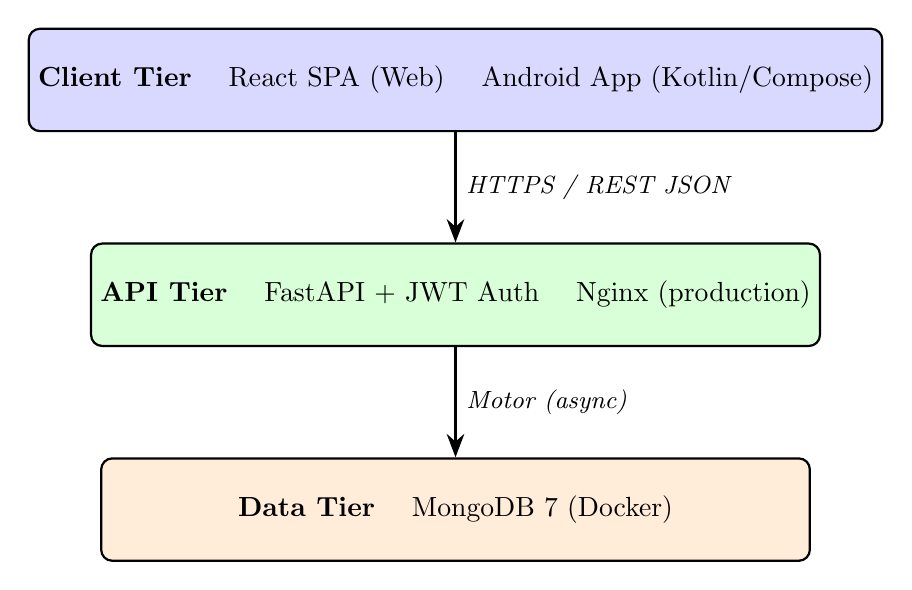
\begin{tikzpicture}[
        node distance=1.4cm,
        box/.style={rectangle, draw=black, thick, minimum width=9cm, minimum height=1.3cm,
                    text centered, rounded corners=4pt, font=\normalsize},
        clientbox/.style={box, fill=blue!15},
        apibox/.style={box, fill=green!15},
        databox/.style={box, fill=orange!15},
        arrow/.style={-Stealth, thick, line width=1.2pt}
    ]
        \node[clientbox] (client) {
            \textbf{Client Tier}~~~
            React SPA (Web) \quad Android App (Kotlin/Compose)
        };
        \node[apibox, below=of client] (api) {
            \textbf{API Tier}~~~
            FastAPI + JWT Auth \quad Nginx (production)
        };
        \node[databox, below=of api] (data) {
            \textbf{Data Tier}~~~
            MongoDB 7 (Docker)
        };
        \draw[arrow] (client) -- node[right, font=\small\itshape]{HTTPS / REST JSON} (api);
        \draw[arrow] (api) -- node[right, font=\small\itshape]{Motor (async)} (data);
    \end{tikzpicture}
    \caption{Three-Tier System Architecture}
    \label{fig:architecture}
\end{figure}

\subsection{Design Principles}

\begin{itemize}
    \item \textbf{RESTful API:} Standard HTTP methods and resource-based URLs with JSON responses
    \item \textbf{Service layer pattern:} Business logic in service classes, separated from API route handlers
    \item \textbf{Component-based frontend:} Modular React components organized by domain
    \item \textbf{Async throughout:} FastAPI async endpoints with async Motor database driver
\end{itemize}

\section{UML Diagrams}

Full UML diagrams are maintained on the project GitHub Wiki at:
\begin{center}
    \url{https://github.com/senaoz/SWE-574/wiki/UML-Diagrams}
\end{center}

The following diagram types are available:

\begin{itemize}
    \item \textbf{Use Case Diagram:} Actors (Regular User, Moderator, Admin) and all major system use cases including service creation, handshake, TimeBank, forum, and communities.
    \item \textbf{Class Diagram:} Key domain entities (User, Service, JoinRequest, Transaction, TimeBank, ChatRoom, ForumDiscussion, ForumEvent, Community, Badge, Rating) and their relationships and cardinalities.
    \item \textbf{Sequence Diagrams:} Step-by-step interaction flows for: (1) service application and approval, (2) transaction completion with TimeBank update, (3) user authentication (JWT issuance and refresh).
\end{itemize}

\section{Scenarios and Mockups}

UI mockups and user scenarios produced during the design phase are available at:
\begin{center}
    \url{https://github.com/senaoz/SWE-574/wiki/Scenarios-\&-Mockups}
\end{center}

Key screens that were mockup'd and implemented:
\begin{itemize}
    \item \textbf{Home page:} Hero section, community values, recent services preview, interactive map
    \item \textbf{Dashboard:} Service grid + map side-by-side, search bar, filters
    \item \textbf{Service Detail:} Full info card, provider profile, location map, apply/chat/save buttons, comments
    \item \textbf{Profile:} Tabs for Services, Applications, Transactions, TimeBank; badge display; ratings
    \item \textbf{Forum:} Discussions/Events tabs; community spaces
    \item \textbf{Admin Panel:} User management, service moderation, analytics
\end{itemize}

\section{Database Design}

\subsection{Collections}

\begin{table}[h]
    \centering
    \begin{tabularx}{\textwidth}{|l|X|}
        \hline
        \textbf{Collection}              & \textbf{Purpose}                                                    \\
        \hline
        \texttt{users}                   & User accounts, profiles, and settings                               \\
        \hline
        \texttt{services}                & Service offers and needs with geolocation                           \\
        \hline
        \texttt{join\_requests}          & Applications from users to services                                 \\
        \hline
        \texttt{transactions}            & Service exchange transactions (dual-confirmation)                   \\
        \hline
        \texttt{timebank\_transactions}  & TimeBank credit audit log                                           \\
        \hline
        \texttt{chat\_rooms}             & Chat room metadata and participant lists                            \\
        \hline
        \texttt{messages}                & Individual chat messages                                            \\
        \hline
        \texttt{saved\_services}         & User bookmarks of services                                          \\
        \hline
        \texttt{forum\_discussions}      & Forum discussion topics                                             \\
        \hline
        \texttt{forum\_events}           & Forum event announcements                                           \\
        \hline
        \texttt{forum\_comments}         & Comments on discussions and events                                  \\
        \hline
        \texttt{communities}             & Community groups and membership                                     \\
        \hline
        \texttt{ratings}                 & Post-exchange star ratings and feedback labels                      \\
        \hline
        \texttt{reports}                 & User-submitted content reports for moderation                       \\
        \hline
        \texttt{notifications}           & In-app notifications (also streamed via SSE)                        \\
        \hline
    \end{tabularx}
    \caption{MongoDB Collections}
\end{table}

\subsection{Key Indexes}

\begin{itemize}
    \item \textbf{Unique:} \texttt{users.email}, \texttt{users.username}
    \item \textbf{Geospatial (2dsphere):} \texttt{services.location} (GeoJSON Point format: \texttt{[longitude, latitude]})
    \item \textbf{Compound unique:} \texttt{saved\_services(user\_id, service\_id)}
    \item \textbf{Partial unique:} \texttt{reports(reported\_by, report\_type, reported\_id)} where \texttt{status = ``pending''}
    \item Standard indexes on \texttt{user\_id}, \texttt{service\_id}, \texttt{status}, \texttt{created\_at} across most collections
\end{itemize}

\section{API Design}

\subsection{RESTful Principles}

\begin{itemize}
    \item Resource-based URLs with standard HTTP methods (GET, POST, PUT, DELETE)
    \item JSON request and response bodies
    \item Standard HTTP status codes
    \item JWT Bearer token authentication on protected routes
\end{itemize}

\subsection{Standard Response Envelope}

\begin{lstlisting}
{
  "data": { ... },
  "message": "Success",
  "status": "success"
}
\end{lstlisting}

\subsection{Authentication}

All protected endpoints require: \texttt{Authorization: Bearer <jwt\_token>}

Token properties: HS256 algorithm, 30-minute expiry, subject = user ID.

Full interactive API documentation: \url{https://backend-swe.gnahh5.easypanel.host/docs}

\section{Frontend Architecture}

\subsection{Routing}

\begin{table}[h]
    \centering
    \begin{tabular}{|l|l|}
        \hline
        \textbf{Route}                                & \textbf{Access}       \\
        \hline
        \texttt{/}                                    & Public                \\
        \hline
        \texttt{/register}                            & Guest only            \\
        \hline
        \texttt{/dashboard}                           & Authenticated user    \\
        \hline
        \texttt{/service/:id}                         & Authenticated user    \\
        \hline
        \texttt{/user/:userId}                        & Authenticated user    \\
        \hline
        \texttt{/profile}                             & Authenticated user    \\
        \hline
        \texttt{/forum}                               & Authenticated user    \\
        \hline
        \texttt{/forum/discussions/:id}               & Authenticated user    \\
        \hline
        \texttt{/forum/events/:id}                    & Authenticated user    \\
        \hline
        \texttt{/forum/communities/:id}               & Authenticated user    \\
        \hline
        \texttt{/forum/communities/:id/posts/:postId} & Authenticated user    \\
        \hline
        \texttt{/settings}                            & Authenticated user    \\
        \hline
        \texttt{/admin}                               & Moderator/Admin only  \\
        \hline
    \end{tabular}
    \caption{Frontend Routes}
\end{table}

\subsection{State Management}

\begin{itemize}
    \item \textbf{React Query:} Server state (all API calls, caching, invalidation)
    \item \textbf{UserContext:} Current user, auth token presence, refetch trigger
    \item \textbf{FilterContext:} Global service search/filter state
    \item \textbf{ThemeContext:} Dark/light mode toggle (persisted to localStorage)
    \item \textbf{localStorage:} JWT access token, theme preference
\end{itemize}

\section{Backend Architecture}

\subsection{Layer Structure}

\begin{itemize}
    \item \textbf{\texttt{api/}:} 15 route handler files --- thin layer delegating to services
    \item \textbf{\texttt{services/}:} Business logic layer --- one class per domain (auth, user, service, transaction, join\_request, chat, comment, forum, community, rating, report, notification, badge, wikidata, content\_moderation)
    \item \textbf{\texttt{models/}:} Pydantic schemas for request/response validation
    \item \textbf{\texttt{core/}:} \texttt{config.py} (settings), \texttt{database.py} (Motor + index creation), \texttt{security.py} (JWT/bcrypt), \texttt{permissions.py} (RBAC)
\end{itemize}

\subsection{RBAC}

Roles: \texttt{user}, \texttt{moderator}, \texttt{admin}, \texttt{banned}.

Dependency functions in \texttt{core/permissions.py}:
\begin{itemize}
    \item \texttt{require\_role([roles])} --- generic role check
    \item \texttt{require\_moderator\_or\_admin()} --- for admin/moderation routes
    \item \texttt{require\_any\_role()} --- any authenticated user
\end{itemize}

% =========================================================
\chapter{Requirement Completion Status}
% =========================================================

\section{Summary}

\begin{table}[h]
    \centering
    \begin{tabular}{|l|c|c|}
        \hline
        \textbf{Category}               & \textbf{Total} & \textbf{Status}       \\
        \hline
        Functional Requirement Groups   & 19             & 19 complete (100\%)   \\
        \hline
        Non-Functional Requirements     & 15             & 13 complete (87\%)    \\
        \hline
        \textbf{Overall}                & \textbf{34}    & \textbf{32 (94\%)}    \\
        \hline
    \end{tabular}
    \caption{Requirement Completion Summary}
\end{table}

Partially completed:
\begin{itemize}
    \item \textbf{NFR--1 (500+ concurrent users):} Architecture supports scaling but load testing not performed.
    \item \textbf{NFR--10 (Daily DB backups):} Manual procedures documented; not automated.
\end{itemize}

\section{Detailed Status}

\begin{longtable}{|p{5.5cm}|p{2cm}|p{6cm}|}
    \hline
    \textbf{Requirement}                 & \textbf{Status}   & \textbf{Notes}                                             \\
    \hline
    \endhead
    FR--1: Authentication                & Complete          & JWT, bcrypt, interest selection on register                \\
    \hline
    FR--2: Profile Management            & Complete          & Tags, bio, profile picture, interests                      \\
    \hline
    FR--3: Offer/Need Management         & Complete          & Full CRUD, capacity, tags, location                        \\
    \hline
    FR--4: Availability                  & Complete          & Duration-based scheduling                                  \\
    \hline
    FR--5: Handshake Mechanism           & Complete          & Join request workflow with full state machine              \\
    \hline
    FR--6: Messaging System              & Complete          & Chat rooms auto-created on approval                        \\
    \hline
    FR--7: TimeBank System               & Complete          & Whole-hour, 10-hour cap, anti-hoarding rule                \\
    \hline
    FR--8: Tagging and Search            & Complete          & Wikidata integration, active-tag filtering                 \\
    \hline
    FR--9: Map Visualization             & Complete          & Google Maps, fuzzed locations, type differentiation        \\
    \hline
    FR--10: Comment and Feedback         & Complete          & Ratings, labels, images, content moderation                \\
    \hline
    FR--11: Reporting and Moderation     & Complete          & Report submission, moderator review, audit log             \\
    \hline
    FR--12: Completion/Transparency      & Complete          & Exchange history on profile                                \\
    \hline
    FR--13: Badges                       & Complete          & 12 badge types, auto-awarded, dynamic recalculation        \\
    \hline
    FR--14: Active Items Management      & Complete          & Profile tabs for services, applications, transactions      \\
    \hline
    FR--15: Community Forum              & Complete          & Discussions, Events, upvotes, comments, pinning            \\
    \hline
    FR--16: User Interaction Features    & Complete          & Save services, share URL                                   \\
    \hline
    FR--17: Mobile-Specific Features     & Complete          & Android app; offline queue, deep links, share sheet        \\
    \hline
    FR--18: Recommendations              & Complete          & Tag-based + proximity scoring                              \\
    \hline
    FR--19: Communities                  & Complete          & Creation, join, posts, events, member management           \\
    \hline
    NFR--1: 500+ concurrent users        & Partial           & Architecture supports it; not load-tested                  \\
    \hline
    NFR--10: Daily DB backups            & Partial           & Procedures documented; not automated                       \\
    \hline
\end{longtable}

% =========================================================
\chapter{System Manual}
% =========================================================

\section{Runtime Requirements}

\subsection{Minimum Requirements}

\begin{itemize}
    \item Docker 20.10+ and Docker Compose 2.0+
    \item 2 GB RAM minimum (4 GB recommended)
    \item 10 GB available disk space
    \item Internet connection (Google Maps API, Wikidata API)
\end{itemize}

\subsection{Production Requirements}

\begin{itemize}
    \item VPS with at least 2 GB RAM
    \item MongoDB 7 (managed or containerized)
    \item Domain name with SSL certificate (HTTPS required)
    \item Google Maps API key
\end{itemize}

\section{Docker Setup}

\subsection{Container Architecture}

Docker Compose orchestrates three containers:

\begin{enumerate}
    \item \textbf{frontend:} React SPA (Vite build) served by Nginx on port 80
    \item \textbf{backend:} FastAPI (Uvicorn) on port 8000
    \item \textbf{mongodb:} MongoDB 7, port 38017 (mapped from internal 27017)
\end{enumerate}

Key files: \texttt{docker-compose.yml}, \texttt{backend/Dockerfile}, \texttt{frontend/Dockerfile}.

\section{Installation Instructions}

\subsection{Quick Start with Docker}

\begin{enumerate}
    \item Clone the repository:
          \begin{lstlisting}[language=bash]
git clone https://github.com/senaoz/SWE-574.git
cd SWE-574
    \end{lstlisting}

    \item Create environment files:
          \begin{lstlisting}[language=bash]
cp backend/.env.example backend/.env
cp frontend/.env.example frontend/.env
    \end{lstlisting}

    \item Edit the \texttt{.env} files with your configuration

    \item Build and start all services:
          \begin{lstlisting}[language=bash]
docker compose up -d --build
    \end{lstlisting}

    \item Access the application:
          \begin{itemize}
              \item Frontend: \url{http://localhost}
              \item Backend API: \url{http://localhost:8000}
              \item API Documentation: \url{http://localhost:8000/docs}
          \end{itemize}
\end{enumerate}

\subsection{Local Backend Development (without Docker)}

Must be run from the \texttt{backend/} directory (relative imports break if run from the project root):

\begin{lstlisting}[language=bash]
cd backend
pip install -r requirements.txt
uvicorn app.main:app --reload --host 0.0.0.0 --port 8000
\end{lstlisting}

\subsection{Local Frontend Development}

\begin{lstlisting}[language=bash]
cd frontend
npm install
npm run dev          # Dev server on port 3000
npm run build        # Production build
npm run type-check   # TypeScript validation
npm test             # Vitest unit tests
\end{lstlisting}

\section{Environment Variables}

\subsection{Backend (\texttt{backend/.env})}

\begin{table}[h]
    \centering
    \begin{tabular}{|l|l|}
        \hline
        \textbf{Variable}        & \textbf{Description}                            \\
        \hline
        \texttt{MONGODB\_URL}    & MongoDB connection string                       \\
        \hline
        \texttt{DATABASE\_NAME}  & Database name                                   \\
        \hline
        \texttt{SECRET\_KEY}     & JWT secret key                                  \\
        \hline
        \texttt{ALLOWED\_ORIGINS}& CORS allowed origins (comma-separated)          \\
        \hline
        \texttt{DEBUG}           & Debug mode flag (\texttt{true}/\texttt{false})  \\
        \hline
    \end{tabular}
    \caption{Backend Environment Variables}
\end{table}

\subsection{Frontend (\texttt{frontend/.env})}

\begin{table}[h]
    \centering
    \begin{tabular}{|l|l|}
        \hline
        \textbf{Variable}          & \textbf{Description}                          \\
        \hline
        \texttt{VITE\_API\_URL}    & Backend API base URL                          \\
        \hline
    \end{tabular}
    \caption{Frontend Environment Variables}
\end{table}

\section{Production Deployment}

\subsection{CI/CD Pipeline}

Deployment is automated via GitHub Actions (\texttt{.github/workflows/deploy-easypanel.yml}). A push to \texttt{main} triggers a deployment webhook to EasyPanel, which pulls the latest code, builds Docker images, and restarts services.

\subsection{EasyPanel Setup}

\begin{enumerate}
    \item Connect the GitHub repository to EasyPanel
    \item Create three services: Frontend (port 80), Backend (port 8000), and MongoDB (managed)
    \item Set all required environment variables
    \item Configure the deployment webhook secret in GitHub Actions secrets
    \item Deploy and verify via \texttt{GET /health} endpoint
\end{enumerate}

% =========================================================
\chapter{User Manual}
% =========================================================

\section{Getting Started}

Navigate to \url{https://swe.gnahh5.easypanel.host} in any modern web browser.

\subsection{Registration}

\begin{enumerate}
    \item Click \textbf{``Sign Up''} on the home page
    \item Fill in: username (unique), email, password (min 8 characters), confirm password, full name
    \item Select at least one interest tag (used for personalized recommendations)
    \item Submit --- you are logged in automatically
\end{enumerate}

\subsection{Login}

\begin{enumerate}
    \item Click \textbf{``Login''}
    \item Enter your email and password
    \item You are redirected to the dashboard
\end{enumerate}

\section{Key Features}

\subsection{Creating a Service}

\begin{enumerate}
    \item Click \textbf{``Create Service''} in the dashboard
    \item Select: \textbf{Offer} (I can provide this) or \textbf{Need} (I need this)
    \item Fill in: title, description, category, duration (whole hours), location, tags
    \item Submit --- service appears on dashboard and map immediately
\end{enumerate}

\subsection{Discovering Services}

\begin{itemize}
    \item \textbf{Dashboard:} Grid of all active services
    \item \textbf{Search bar:} Keyword search across title, description, and tags
    \item \textbf{Filters:} Narrow by category, city, or service type
    \item \textbf{Interactive map:} Click markers to see service previews
    \item \textbf{Recommendations:} ``Recommended for You'' section based on interests
\end{itemize}

\subsection{Applying to a Service}

\begin{enumerate}
    \item Click on a service card to view details
    \item Click \textbf{``Apply''} and optionally add a message
    \item Your request shows ``Pending'' status in Profile \textrightarrow{} Applications
\end{enumerate}

\subsection{Managing Join Requests (as Provider)}

\begin{enumerate}
    \item Go to Profile \textrightarrow{} Services tab, open your service
    \item View the Applicants section and review applicant profiles
    \item Approve or reject each application
    \item On approval: transaction is created automatically; chat room opens
\end{enumerate}

\subsection{Completing Transactions}

Both parties must confirm:

\begin{enumerate}
    \item Go to Profile \textrightarrow{} Transactions tab
    \item Click \textbf{``Confirm Completion''} on the active transaction
    \item When both parties confirm: transaction finalizes, TimeBank balances update, rating form unlocks
\end{enumerate}

\subsection{Using Chat}

\begin{enumerate}
    \item Navigate to the Chat page or click \textbf{``Chat''} on any service detail page
    \item Select a room from the sidebar and type/send messages
    \item Chat rooms are automatically linked to services or transactions
\end{enumerate}

\subsection{TimeBank System}

\begin{itemize}
    \item Starting balance: 3 hours; maximum: 10 hours
    \item Only whole-hour transactions supported
    \item When you reach 10 hours, you must post a Need to earn more
    \item View your balance and full history in Profile \textrightarrow{} TimeBank tab
\end{itemize}

\subsection{Forum and Communities}

\begin{itemize}
    \item \textbf{Forum Discussions:} Create threads, comment, upvote; search by keyword or tag
    \item \textbf{Forum Events:} Announce events with date/time; mark attendance
    \item \textbf{Communities:} Join groups, contribute posts, view unified community feed
\end{itemize}

\subsection{Profile and Badges}

\begin{itemize}
    \item Your profile shows completed exchanges, ratings, interest tags, and earned badges
    \item Badges are awarded automatically (e.g., ``Honey Maker'' for first completed exchange)
    \item Update profile, interests, and profile picture in Settings
\end{itemize}

% =========================================================
\chapter{API Documentation}
% =========================================================

\section{Overview}

The Hive Platform backend exposes a RESTful API. Full interactive documentation (Swagger UI):
\begin{center}
    \url{https://backend-swe.gnahh5.easypanel.host/docs}
\end{center}

\subsection{Authentication}

All protected endpoints require:
\begin{lstlisting}
Authorization: Bearer <access_token>
\end{lstlisting}
Tokens are obtained via \texttt{POST /login}. Expiry: 30 minutes.

\subsection{Response Format}

\begin{lstlisting}
{
  "data": { ... },
  "message": "Success",
  "status": "success"
}
\end{lstlisting}

\section{Endpoint Reference}

\subsection{Authentication}

\begin{longtable}{|l|p{4.5cm}|p{5cm}|l|}
    \hline
    \textbf{Method} & \textbf{Path}              & \textbf{Description}            & \textbf{Auth} \\
    \hline
    \endhead
    POST            & \texttt{/register}         & Register a new user             & No            \\
    \hline
    POST            & \texttt{/login}            & Login; returns JWT token        & No            \\
    \hline
    GET             & \texttt{/me}               & Get current user info           & Yes           \\
    \hline
\end{longtable}

\subsection{Users}

\begin{longtable}{|l|p{4.5cm}|p{5cm}|l|}
    \hline
    \textbf{Method} & \textbf{Path}                          & \textbf{Description}                & \textbf{Auth} \\
    \hline
    \endhead
    GET             & \texttt{/profile}                      & Get own profile                     & Yes           \\
    \hline
    PUT             & \texttt{/profile}                      & Update own profile                  & Yes           \\
    \hline
    GET             & \texttt{/timebank}                     & Get TimeBank balance + history      & Yes           \\
    \hline
    GET             & \texttt{/badges}                       & Get own badges                      & Yes           \\
    \hline
    GET             & \texttt{/settings}                     & Get user settings                   & Yes           \\
    \hline
    PUT             & \texttt{/settings}                     & Update user settings                & Yes           \\
    \hline
    POST            & \texttt{/change-password}              & Change password                     & Yes           \\
    \hline
    GET             & \texttt{/search}                       & Search users                        & Yes           \\
    \hline
    GET             & \texttt{/\{user\_id\}}                 & Get public profile by ID            & Yes           \\
    \hline
    GET             & \texttt{/\{user\_id\}/badges}          & Get badges for a user               & Yes           \\
    \hline
    PUT             & \texttt{/\{user\_id\}/role}            & Update user role                    & Admin         \\
    \hline
\end{longtable}

\subsection{Services}

\begin{longtable}{|l|p{4.5cm}|p{5cm}|l|}
    \hline
    \textbf{Method} & \textbf{Path}                          & \textbf{Description}                & \textbf{Auth} \\
    \hline
    \endhead
    GET             & \texttt{/services}                     & List/search services                & Yes           \\
    \hline
    POST            & \texttt{/services}                     & Create a service                    & Yes           \\
    \hline
    GET             & \texttt{/services/saved}               & Get saved services                  & Yes           \\
    \hline
    GET             & \texttt{/services/recommendations}     & Get personalized recommendations    & Yes           \\
    \hline
    GET             & \texttt{/services/\{id\}}              & Get service details                 & Yes           \\
    \hline
    PUT             & \texttt{/services/\{id\}}              & Update a service                    & Yes           \\
    \hline
    DELETE          & \texttt{/services/\{id\}}              & Delete a service                    & Yes           \\
    \hline
    POST            & \texttt{/services/\{id\}/save}         & Save a service                      & Yes           \\
    \hline
    POST            & \texttt{/services/\{id\}/complete}     & Mark service complete               & Yes           \\
    \hline
    POST            & \texttt{/services/\{id\}/cancel}       & Cancel a service                    & Yes           \\
    \hline
\end{longtable}

\subsection{Join Requests}

\begin{longtable}{|l|p{4.5cm}|p{5cm}|l|}
    \hline
    \textbf{Method} & \textbf{Path}                               & \textbf{Description}            & \textbf{Auth} \\
    \hline
    \endhead
    POST            & \texttt{/join-requests}                     & Apply to a service              & Yes           \\
    \hline
    GET             & \texttt{/join-requests/my-requests}         & Get own join requests           & Yes           \\
    \hline
    GET             & \texttt{/join-requests/service/\{id\}}      & List requests for a service     & Yes           \\
    \hline
    PUT             & \texttt{/join-requests/\{id\}}              & Approve or reject a request     & Yes           \\
    \hline
    POST            & \texttt{/join-requests/\{id\}/cancel}       & Cancel own pending request      & Yes           \\
    \hline
\end{longtable}

\subsection{Transactions}

\begin{longtable}{|l|p{4.5cm}|p{5cm}|l|}
    \hline
    \textbf{Method} & \textbf{Path}                                     & \textbf{Description}              & \textbf{Auth} \\
    \hline
    \endhead
    POST            & \texttt{/transactions}                            & Create a transaction              & Yes           \\
    \hline
    GET             & \texttt{/transactions/my-transactions}            & Get own transactions              & Yes           \\
    \hline
    POST            & \texttt{/transactions/\{id\}/confirm-completion}  & Confirm transaction complete      & Yes           \\
    \hline
    GET             & \texttt{/transactions/\{id\}}                     & Get transaction details           & Yes           \\
    \hline
\end{longtable}

\subsection{Chat}

\begin{longtable}{|l|p{4.5cm}|p{5cm}|l|}
    \hline
    \textbf{Method} & \textbf{Path}                           & \textbf{Description}             & \textbf{Auth} \\
    \hline
    \endhead
    GET             & \texttt{/chat/rooms}                    & List chat rooms                  & Yes           \\
    \hline
    POST            & \texttt{/chat/rooms}                    & Create a chat room               & Yes           \\
    \hline
    GET             & \texttt{/chat/rooms/\{id\}}             & Get room details                 & Yes           \\
    \hline
    GET             & \texttt{/chat/rooms/\{id\}/messages}    & Get room message history         & Yes           \\
    \hline
    POST            & \texttt{/chat/messages}                 & Send a message                   & Yes           \\
    \hline
    DELETE          & \texttt{/chat/messages/\{id\}}          & Delete a message                 & Yes           \\
    \hline
\end{longtable}

\subsection{Forum}

\begin{longtable}{|l|p{4.5cm}|p{5cm}|l|}
    \hline
    \textbf{Method} & \textbf{Path}                                  & \textbf{Description}           & \textbf{Auth} \\
    \hline
    \endhead
    GET             & \texttt{/forum/discussions}                    & List discussions               & Yes           \\
    \hline
    POST            & \texttt{/forum/discussions}                    & Create a discussion            & Yes           \\
    \hline
    GET             & \texttt{/forum/discussions/\{id\}}             & Get discussion details         & Yes           \\
    \hline
    PUT             & \texttt{/forum/discussions/\{id\}}             & Update a discussion            & Yes           \\
    \hline
    DELETE          & \texttt{/forum/discussions/\{id\}}             & Delete a discussion            & Yes           \\
    \hline
    POST            & \texttt{/forum/discussions/\{id\}/upvote}      & Upvote a discussion            & Yes           \\
    \hline
    GET             & \texttt{/forum/events}                         & List events                    & Yes           \\
    \hline
    POST            & \texttt{/forum/events}                         & Create an event                & Yes           \\
    \hline
    POST            & \texttt{/forum/events/\{id\}/attend}           & Mark attendance for event      & Yes           \\
    \hline
    POST            & \texttt{/forum/comments}                       & Post a comment                 & Yes           \\
    \hline
    POST            & \texttt{/forum/comments/\{id\}/upvote}         & Upvote a comment               & Yes           \\
    \hline
\end{longtable}

\subsection{Communities}

\begin{longtable}{|l|p{4.5cm}|p{5cm}|l|}
    \hline
    \textbf{Method} & \textbf{Path}                                   & \textbf{Description}          & \textbf{Auth} \\
    \hline
    \endhead
    GET             & \texttt{/communities}                           & List communities              & Yes           \\
    \hline
    POST            & \texttt{/communities}                           & Create a community            & Yes           \\
    \hline
    GET             & \texttt{/communities/my}                        & Get my communities            & Yes           \\
    \hline
    GET             & \texttt{/communities/\{id\}}                    & Get community details         & Yes           \\
    \hline
    POST            & \texttt{/communities/\{id\}/join}               & Join a community              & Yes           \\
    \hline
    DELETE          & \texttt{/communities/\{id\}/leave}              & Leave a community             & Yes           \\
    \hline
    GET             & \texttt{/communities/\{id\}/posts}              & List community posts          & Yes           \\
    \hline
    POST            & \texttt{/communities/\{id\}/posts}              & Create a post in community    & Yes           \\
    \hline
    POST            & \texttt{/communities/\{id\}/posts/\{pid\}/upvote} & Upvote a community post     & Yes           \\
    \hline
\end{longtable}

\subsection{Ratings}

\begin{longtable}{|l|p{4.5cm}|p{5cm}|l|}
    \hline
    \textbf{Method} & \textbf{Path}                                 & \textbf{Description}         & \textbf{Auth} \\
    \hline
    \endhead
    POST            & \texttt{/ratings}                             & Submit a rating              & Yes           \\
    \hline
    GET             & \texttt{/ratings/user/\{user\_id\}}           & Get ratings for a user       & Yes           \\
    \hline
    GET             & \texttt{/ratings/transaction/\{id\}}          & Get ratings for transaction  & Yes           \\
    \hline
\end{longtable}

\subsection{Notifications}

\begin{longtable}{|l|p{4.5cm}|p{5cm}|l|}
    \hline
    \textbf{Method} & \textbf{Path}                               & \textbf{Description}           & \textbf{Auth} \\
    \hline
    \endhead
    GET             & \texttt{/notifications/stream}              & SSE stream for live updates    & Yes           \\
    \hline
    GET             & \texttt{/notifications/unread-count}        & Get unread notification count  & Yes           \\
    \hline
    GET             & \texttt{/notifications}                     & List notifications             & Yes           \\
    \hline
    PUT             & \texttt{/notifications/read-all}            & Mark all notifications as read & Yes           \\
    \hline
    PUT             & \texttt{/notifications/\{id\}/read}         & Mark one notification as read  & Yes           \\
    \hline
\end{longtable}

\subsection{Admin}

\begin{longtable}{|l|p{4.5cm}|p{5cm}|l|}
    \hline
    \textbf{Method} & \textbf{Path}                                      & \textbf{Description}           & \textbf{Auth} \\
    \hline
    \endhead
    GET             & \texttt{/admin/db/stats}                           & Database statistics            & Admin         \\
    \hline
    GET             & \texttt{/admin/failed-transactions}                & Failed TimeBank transactions   & Admin         \\
    \hline
    GET             & \texttt{/admin/analytics/service-participation}    & Participation analytics        & Admin         \\
    \hline
\end{longtable}

\subsection{File Uploads}

Files are uploaded via \texttt{multipart/form-data} to \texttt{/upload/\{type\}} and served as static files at \texttt{/uploads/\{type\}/\{filename\}}. Supported types: \texttt{profile}, \texttt{services}, \texttt{communities}, \texttt{ratings}, \texttt{comments}, \texttt{forum-events}, \texttt{discussions}.

% =========================================================
\chapter{Test Plan and Results}
\label{chap:tests}
% =========================================================

\section{Test Strategy}

The Hive Platform uses a multi-layered testing approach:

\begin{enumerate}
    \item \textbf{Unit Tests:} Individual service and API components tested in isolation using mongomock
    \item \textbf{Integration Tests:} API endpoints tested via FastAPI TestClient
    \item \textbf{User Acceptance Tests:} End-to-end scenarios executed manually on the deployed system
\end{enumerate}

\subsection{Testing Framework}

\begin{itemize}
    \item \textbf{Backend:} pytest with pytest-asyncio
    \item \textbf{Mock Database:} mongomock with custom async wrapper (no real MongoDB needed)
    \item \textbf{API Testing:} FastAPI TestClient
    \item \textbf{Coverage:} pytest-cov (generates HTML report in \texttt{backend/htmlcov/})
    \item \textbf{Frontend:} Vitest with jsdom
\end{itemize}

\section{Unit Test Suite}

\subsection{Running Tests}

\begin{lstlisting}[language=bash]
cd backend
pytest tests/ -v                          # All tests
pytest tests/ --cov=app --cov-report=html # With HTML coverage report
pytest tests/test_auth_api.py -v          # Single file
pytest tests/test_auth_api.py::test_fn -v # Single function
\end{lstlisting}

\subsection{Test Files}

The backend test suite contains \textbf{33 test files} covering all major API and service modules:

\begin{table}[h]
    \centering
    \begin{tabular}{|l|l|}
        \hline
        \textbf{Test File}                     & \textbf{Coverage Area}           \\
        \hline
        \texttt{test\_auth\_api.py}            & Authentication API endpoints     \\
        \hline
        \texttt{test\_auth\_service.py}        & Authentication service layer     \\
        \hline
        \texttt{test\_services\_api.py}        & Services API endpoints           \\
        \hline
        \texttt{test\_service\_service.py}     & Services business logic          \\
        \hline
        \texttt{test\_users\_api.py}           & Users API endpoints              \\
        \hline
        \texttt{test\_user\_service.py}        & Users service layer              \\
        \hline
        \texttt{test\_transactions\_api.py}    & Transactions API endpoints       \\
        \hline
        \texttt{test\_transaction\_service.py} & Transaction business logic       \\
        \hline
        \texttt{test\_join\_requests\_api.py}  & Join Requests API endpoints      \\
        \hline
        \texttt{test\_join\_request\_service.py} & Join request business logic    \\
        \hline
        \texttt{test\_chat\_api.py}            & Chat API endpoints               \\
        \hline
        \texttt{test\_chat\_service.py}        & Chat service layer               \\
        \hline
        \texttt{test\_forum\_api.py}           & Forum API endpoints              \\
        \hline
        \texttt{test\_forum\_service.py}       & Forum service layer              \\
        \hline
        \texttt{test\_community\_service.py}   & Community service layer          \\
        \hline
        \texttt{test\_comments\_api.py}        & Comments API endpoints           \\
        \hline
        \texttt{test\_comment\_service.py}     & Comment service layer            \\
        \hline
        \texttt{test\_ratings\_api.py}         & Ratings API endpoints            \\
        \hline
        \texttt{test\_rating\_service.py}      & Rating service layer             \\
        \hline
        \texttt{test\_notification\_api.py}    & Notifications API endpoints      \\
        \hline
        \texttt{test\_notification\_service.py}& Notification service layer       \\
        \hline
        \texttt{test\_badge\_service.py}       & Badge auto-award logic           \\
        \hline
        \texttt{test\_report\_service.py}      & Report and moderation logic      \\
        \hline
        \texttt{test\_pinning\_api.py}         & Content pinning API              \\
        \hline
        \texttt{test\_balance\_controls.py}    & TimeBank balance enforcement     \\
        \hline
        \texttt{test\_timebank\_dedup.py}      & TimeBank deduplication logic     \\
        \hline
        \texttt{test\_upload\_api.py}          & File upload endpoints            \\
        \hline
        \texttt{test\_security.py}             & Security and JWT functions       \\
        \hline
        \texttt{test\_wikidata.py}             & Wikidata API integration         \\
        \hline
        \texttt{test\_admin\_api.py}           & Admin API endpoints              \\
        \hline
    \end{tabular}
    \caption{Backend Test Files}
\end{table}

\subsection{Test Environment}

\begin{itemize}
    \item \textbf{Database:} mongomock (no real MongoDB required)
    \item \textbf{Auth:} Mock JWT tokens defined in \texttt{conftest.py}
    \item \textbf{Fixtures:} Shared mock DB, TestClient, sample users/services, auth headers defined in \texttt{conftest.py}
    \item \textbf{Execution:} Fast --- no database cleanup needed between tests
\end{itemize}

\section{User Acceptance Tests}

Ten end-to-end scenarios were executed manually on the deployed system. All 10 scenarios passed.

\begin{table}[h]
    \centering
    \begin{tabular}{|l|l|l|}
        \hline
        \textbf{Scenario}                          & \textbf{Objective}                             & \textbf{Result} \\
        \hline
        1. Registration and Login                  & Create account and authenticate                & Passed          \\
        \hline
        2. Create Service Offer                    & Create offer visible on dashboard and map      & Passed          \\
        \hline
        3. Discover and Apply to Service           & Search, view, submit join request              & Passed          \\
        \hline
        4. Approve Request, Create Transaction     & Provider approves; auto transaction created    & Passed          \\
        \hline
        5. Complete Transaction                    & Dual confirmation; TimeBank update             & Passed          \\
        \hline
        6. Chat Communication                      & Messages visible to both participants          & Passed          \\
        \hline
        7. Search and Filtering                    & Filters work; map updates dynamically          & Passed          \\
        \hline
        8. Forum and Communities                   & Discussions, events, upvotes, community posts  & Passed          \\
        \hline
        9. Admin Panel                             & Admin features accessible; moderation works    & Passed          \\
        \hline
        10. Responsive Design                      & Mobile and desktop layouts verified            & Passed          \\
        \hline
    \end{tabular}
    \caption{User Acceptance Test Results}
\end{table}

% =========================================================
\chapter{Use Case Demo}
\label{chap:usecase}
% =========================================================

\section{End-to-End Exchange Scenario}

This chapter demonstrates a complete service exchange from creation to completion and TimeBank credit transfer.

\subsection{Actors}

\begin{itemize}
    \item \textbf{Ayse} (Requester): Graphic designer who needs gardening help. Balance: 3 hours.
    \item \textbf{Mehmet} (Provider): Experienced gardener offering services. Balance: 3 hours.
\end{itemize}

\subsection{Preconditions}

Both users are registered and logged in with their starting TimeBank balance of 3 hours.

\section{Step-by-Step Flow}

\subsection{Phase 1: Service Creation (Mehmet)}

\begin{enumerate}
    \item Mehmet clicks \textbf{``Create Service''} and selects \textbf{Offer}
    \item Fills in: title ``Professional Gardening Help'', duration 2 hours, location Istanbul, tags: gardening, outdoor
    \item Submits --- service appears on dashboard and map with ``active'' status
\end{enumerate}

\subsection{Phase 2: Service Discovery (Ayse)}

\begin{enumerate}
    \item Ayse searches ``gardening'' on the dashboard
    \item Finds Mehmet's service card and opens the detail page
\end{enumerate}

\subsection{Phase 3: Application (Ayse)}

\begin{enumerate}
    \item Ayse clicks \textbf{``Apply''} and adds message: ``I need help with my backyard. Available weekends.''
    \item Join request created with ``pending'' status
    \item Status visible in Profile \textrightarrow{} Applications tab
\end{enumerate}

\subsection{Phase 4: Approval (Mehmet)}

\begin{enumerate}
    \item Mehmet goes to Profile \textrightarrow{} Services \textrightarrow{} Applicants
    \item Reviews Ayse's profile and clicks \textbf{``Approve''}
    \item System automatically creates a transaction and opens a chat room
    \item Service status changes to ``in\_progress''
\end{enumerate}

\subsection{Phase 5: Coordination via Chat}

Both users exchange messages in the auto-created chat room to confirm meeting details.

\subsection{Phase 6: Completion}

\begin{enumerate}
    \item Mehmet goes to Profile \textrightarrow{} Transactions and clicks \textbf{``Confirm Completion''}
    \item Transaction shows ``waiting for requester confirmation''
    \item Ayse confirms --- transaction finalizes automatically
    \item \textbf{Mehmet's balance:} 3 + 2 = \textbf{5 hours}
    \item \textbf{Ayse's balance:} 3 - 2 = \textbf{1 hour}
\end{enumerate}

\subsection{Phase 7: Post-Exchange}

Both users can now leave a rating and comment on each other's profiles.

% =========================================================
\chapter{References}
% =========================================================

\section{Technical Documentation}

\begin{itemize}
    \item FastAPI Documentation: \url{https://fastapi.tiangolo.com/}
    \item React Documentation: \url{https://react.dev/}
    \item MongoDB Documentation: \url{https://www.mongodb.com/docs/}
    \item Radix UI: \url{https://www.radix-ui.com/}
    \item Google Maps Platform: \url{https://developers.google.com/maps}
    \item Wikidata: \url{https://www.wikidata.org/}
    \item Docker Documentation: \url{https://docs.docker.com/}
    \item IEEE 830-1998 --- IEEE Recommended Practice for Software Requirements Specifications
\end{itemize}

\section{Project Resources}

\begin{itemize}
    \item Repository: \url{https://github.com/senaoz/SWE-574}
    \item Live Application: \url{https://swe.gnahh5.easypanel.host}
    \item Backend API Docs: \url{https://backend-swe.gnahh5.easypanel.host/docs}
    \item GitHub Wiki: \url{https://github.com/senaoz/SWE-574/wiki}
    \item UML Diagrams: \url{https://github.com/senaoz/SWE-574/wiki/UML-Diagrams}
    \item Scenarios \& Mockups: \url{https://github.com/senaoz/SWE-574/wiki/Scenarios-\&-Mockups}
    \item Milestone 1 Report: \url{https://github.com/senaoz/SWE-574/blob/main/reports/m1\_group3.md}
    \item Milestone 2 Report: \url{https://github.com/senaoz/SWE-574/blob/main/reports/m2\_group3.md}
\end{itemize}

% =========================================================
\chapter{Conclusion}
% =========================================================

\section{Project Summary}

The Hive Platform has been successfully designed, developed, tested, and deployed as a production system. All 19 functional requirement groups are fully implemented and all 10 user acceptance test scenarios passed. The platform is operational at \url{https://swe.gnahh5.easypanel.host} and ready for evaluation.

\section{Key Achievements}

\begin{itemize}
    \item Complete service exchange workflow from posting to TimeBank credit transfer
    \item Privacy-preserving interactive map with fuzzed coordinates (Google Maps API)
    \item Community forum with discussions, events, upvotes, pinning, and communities
    \item Automated badge system with 12 badge types based on objective criteria
    \item Post-exchange ratings with star scores, labeled feedback, and image attachments
    \item Personalized recommendation engine using interest tags, activity signals, and geoproximity
    \item Content moderation via automated profanity filter and moderator review workflow
    \item Server-Sent Events (SSE) for real-time in-app notifications
    \item Native Android application (Kotlin/Jetpack Compose) sharing the same backend
    \item 33 automated test files covering all major API and service modules
    \item Full CI/CD pipeline via GitHub Actions to EasyPanel production deployment
\end{itemize}

\section{Future Enhancements}

\begin{itemize}
    \item Automated database backup procedures (NFR--10)
    \item Load testing to verify 500+ concurrent user support (NFR--1)
    \item WebSocket-based real-time chat (currently polling)
    \item Email notifications for critical events
    \item Calendar-based service availability scheduling
    \item Advanced ML-based recommendation improvements
\end{itemize}

\section{Final Statement}

The Hive Platform represents a complete implementation of a community service exchange system based on the TimeBank concept. The project demonstrates proficiency in full-stack web development (React, FastAPI, MongoDB), mobile development (Android/Kotlin), software engineering practices (RBAC, geospatial queries, content moderation, CI/CD), and systematic project management from requirements through production deployment.

\end{document}
